
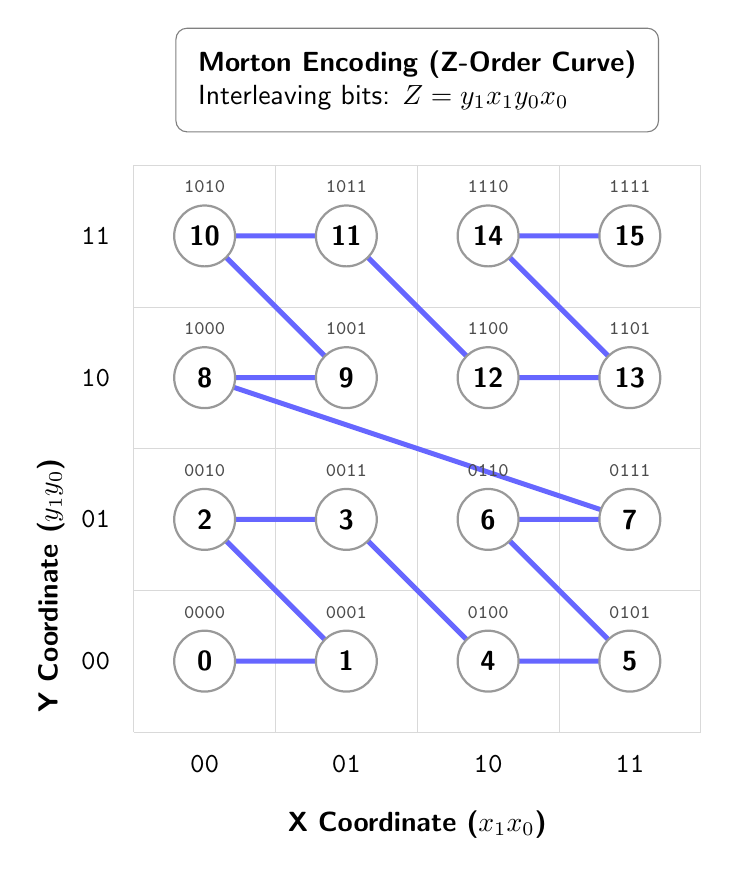
\begin{tikzpicture}[scale=1.8, font=\sffamily]

    % 1. Draw the background grid
    \draw[step=1cm, gray!30, very thin] (0,0) grid (4,4);

    % 2. Draw axis labels (Binary Coordinates)
    \foreach \x/\label in {0.5/00, 1.5/01, 2.5/10, 3.5/11} {
        \node[below=5pt] at (\x, 0) {\texttt{\label}};
    }
    \foreach \y/\label in {0.5/00, 1.5/01, 2.5/10, 3.5/11} {
        \node[left=5pt] at (0, \y) {\texttt{\label}};
    }
    
    % Axis Titles
    \node[below=25pt] at (2,0) {\textbf{X Coordinate ($x_1 x_0$)}};
    \node[left=30pt, rotate=90] at (0,2) {\textbf{Y Coordinate ($y_1 y_0$)}};

    % 3. Define the coordinates for the Z-curve path 
    % Z-value = interleaved bits: y_1 x_1 y_0 x_0
    \foreach \x/\y/\dec in {
        0.5/0.5/0,  1.5/0.5/1,  0.5/1.5/2,  1.5/1.5/3,
        2.5/0.5/4,  3.5/0.5/5,  2.5/1.5/6,  3.5/1.5/7,
        0.5/2.5/8,  1.5/2.5/9,  0.5/3.5/10, 1.5/3.5/11,
        2.5/2.5/12, 3.5/2.5/13, 2.5/3.5/14, 3.5/3.5/15%
    } {
        \node[coordinate] (P\dec) at (\x,\y) {};
    }

    % 4. Draw the actual Z-curve connecting the points
    \draw[->, color=blue!60, line width=1.8pt, rounded corners=3pt]
        (P0) -- (P1) -- (P2) -- (P3) --
        (P4) -- (P5) -- (P6) -- (P7) --
        (P8) -- (P9) -- (P10) -- (P11) --
        (P12) -- (P13) -- (P14) -- (P15);

    % 5. Draw the nodes on top of the line for clarity
    % Includes the Decimal value (circle) and Binary Interleaved value (above)
    \foreach \x/\y/\dec/\bin in {
        0.5/0.5/0/0000, 1.5/0.5/1/0001, 0.5/1.5/2/0010, 1.5/1.5/3/0011,
        2.5/0.5/4/0100, 3.5/0.5/5/0101, 2.5/1.5/6/0110, 3.5/1.5/7/0111,
        0.5/2.5/8/1000, 1.5/2.5/9/1001, 0.5/3.5/10/1010, 1.5/3.5/11/1011,
        2.5/2.5/12/1100, 3.5/2.5/13/1101, 2.5/3.5/14/1110, 3.5/3.5/15/1111%
    } {
        % Decimal Node
        \node[circle, fill=white, draw=gray!80, thick, minimum size=22pt, inner sep=0pt] 
            at (\x,\y) {\textbf{\dec}};
        
        % Binary Interleaved Node
        \node[above=12pt, font=\scriptsize, color=black!70] 
            at (\x,\y) {\texttt{\bin}};
    }
    
    % 6. Add a legend/title box
    \node[draw=gray, fill=white, align=left, rounded corners, inner sep=8pt] 
        at (2, 4.6) {
        \textbf{Morton Encoding (Z-Order Curve)} \\
        Interleaving bits: $Z = y_1 x_1 y_0 x_0$
    };

\end{tikzpicture}